\documentclass[class=jsarticle, crop=false, dvipdfmx, fleqn]{standalone}
\input{/Users/User/Documents/University/report_template/preamble/preamble}
\begin{document}

\section*{宿題1}

2つの正規分布にそれぞれ従う2次元点群を2セット用意し,
正規分布のパラメータを既知として識別関数を設計して,
これらの点群を分類する。
識別関数は,
\begin{itemize}
    \item Case 1: \(\bm{\Sigma}_i = \sigma^2 \bm{I}\)
    \item Case 2: \(\bm{\Sigma}_i = \bm{\sigma}\)
    \item Case 3: \(\bm{\Sigma}_i = \text{arbitrary}\)
\end{itemize}
の3ケースについて考える。



\subsection*{理論}

ガウスモデル
\begin{equation}
    p(\bm{x}|y) = \frac{1}{(2\pi)^{d/2} \det(\bm{\Sigma})^{1/2}} \exp(-\frac{1}{2} (\bm{x} - \bm{\mu})^\mathrm{T} \bm{\Sigma}^{-1} (\bm{x} - \bm{\mu}))
\end{equation}
を考えると,
ベイズの定理より,
\begin{align}
    p(y|\bm{x}) & = \frac{p(\bm{x}|y) p(y)}{p(\bm{x})} \\
    \log(p(y|\bm{x}))
        & = \log(p(x|y)) + \log(p(y)) - \log(p(x)) \\
        & = -\frac{d}{2} \log(2 \pi) - \frac{1}{2} \log(\det(\bm{\Sigma})) - \frac{1}{2} (\bm{x} - \bm{\mu})^\mathrm{T} \bm{\Sigma}^{-1} (\bm{x} - \bm{\mu}) + \log(p(y)) - \log(p(\bm{x})) \\
        & = - \frac{1}{2} (\bm{x} - \bm{\mu})^\mathrm{T} \bm{\Sigma}^{-1} (\bm{x} - \bm{\mu}) + \log(p(y)) - \frac{1}{2} \log(\det(\bm{\Sigma})) + \log(p(y)) + C
        \label{eq:log_prob_y_given_x} \\
    C & = -\frac{d}{2} \log(2 \pi) - \log(p(\bm{x}))
\end{align}
となる。
いま,二値分類を考えると,識別関数\(g\)は,
\begin{align}
    g(\bm{x})
        & = \log(p(y=1|\bm{x})) - \log(p(y=2|\bm{x})) \\
        & = -\frac{1}{2} \qty((\bm{x} - \bm{\mu}_1)^\mathrm{T} \bm{\Sigma}_1^{-1} (\bm{x} - \bm{\mu}_1) - (\bm{x} - \bm{\mu}_2)^\mathrm{T} \bm{\Sigma}_2^{-1} (\bm{x} - \bm{\mu}_2)) - \frac{1}{2} \log(\frac{\det(\bm{\Sigma}_1)}{\det(\bm{\Sigma}_2)}) + \log(\frac{p_1}{p_2})
        \label{eq:classifier}
\end{align}
となる。この\(g\)が正であれば予測は1,負なら2である。

Case 1のとき,\(\bm{\Sigma}_1 = \bm{\Sigma}_2 = \sigma^2 \bm{I}\)から,
\begin{equation}
    g(\bm{x}) =
        \frac{1}{\sigma^2} (\bm{\mu}_1 - \bm{\mu}_2)^\mathrm{T} \bm{x}
        + \qty(-\frac{1}{2}(||\bm{\mu}_1||^2 - ||\bm{\mu}_2||^2) + \log(\frac{p_1}{p_2}))
\end{equation}

Case 2のとき,\(\bm{\Sigma}_1 = \bm{\Sigma}_2 = \Sigma\)から,
\begin{equation}
    g(\bm{x}) =
        \bm{\Sigma}^{-1} (\bm{\mu}_1 - \bm{\mu}_2)^\mathrm{T} \bm{x}
        + \qty(-\frac{1}{2}(\bm{\mu}_1^\mathrm{T} \bm{\Sigma}^{-1} \bm{\mu}_1 - \bm{\mu}_2^\mathrm{T} \bm{\Sigma}^{-1} \bm{\mu}_2) + \log(\frac{p_1}{p_2}))
\end{equation}

Case 3のとき,
\begin{align}
    g(\bm{x})
        & =
        - \frac{1}{2} \bm{x}^\mathrm{T} (\bm{\Sigma}_1^{-1} - \bm{\Sigma}_2^{-1}) \bm{x}
        + (\bm{\mu}_1^\mathrm{T} \bm{\Sigma}_1^{-1} - \bm{\mu}_2^\mathrm{T} \bm{\Sigma}_2^{-1}) \bm{x}
        \notag \\ & \qquad
        + \qty(
            \bm{\mu}_1^\mathrm{T} \bm{\Sigma}_1^{-1} \bm{\mu}_1 - \bm{\mu}_2^\mathrm{T} \bm{\Sigma}_1^{-1} \bm{\mu}_2
            - \frac{1}{2} \log(\frac{\det(\bm{\Sigma}_1)}{\det(\bm{\Sigma}_2)})
            + \log(\frac{p_1}{p_2})
            )
\end{align}



\subsection*{条件設定}

2つの正規分布にそれぞれ従う2次元点群(以下ではdatasetと呼ぶ)は3種類用意した。
それぞれの概要は表\ref{tab:datasets}にまとめた。

\begin{table}
    \centering
    \caption{3つのdatasetの概要}
    \begin{tabular}{lccc} \hline
        dataset & 1 & 2 & 3 \\ \hline
        総点数 & 1000 & 1000 & 1000 \\ \hline
        点群1に属する点の数 & 307 & 415 & 517 \\ \hline
        点群2に属する点の数 & 693 & 585 & 483 \\ \hline
        点群1の平均
            & \(\begin{bmatrix} 2 \\ 0 \end{bmatrix}\)
            & \(\begin{bmatrix} 2 \\ 2 \end{bmatrix}\)
            & \(\begin{bmatrix} 1 \\ 1 \end{bmatrix}\) \\ \hline
        点群2の平均
            & \(\begin{bmatrix} -2 \\ 0 \end{bmatrix}\)
            & \(\begin{bmatrix} -2 \\ -2 \end{bmatrix}\)
            & \(\begin{bmatrix} 1 \\ 1 \end{bmatrix}\) \\ \hline
        点群1の共分散行列
            & \(\begin{bmatrix} 1 & 0 \\ 0 & 9 \end{bmatrix}\)
            & \(\begin{bmatrix} 5 & 0 \\ 0 & 6 \end{bmatrix}\)
            & \(\begin{bmatrix} 1 & 0 \\ 0 & 2 \end{bmatrix}\) \\ \hline
        点群2の共分散行列
            & \(\begin{bmatrix} 1 & 0 \\ 0 & 2 \end{bmatrix}\)
            & \(\begin{bmatrix} 6 & 0 \\ 0 & 4 \end{bmatrix}\)
            & \(\begin{bmatrix} 8 & 0 \\ 0 & 5 \end{bmatrix}\) \\ \hline
    \end{tabular}
    \label{tab:datasets}
\end{table}



\subsection*{プログラム}

プログラムの本体は\pageref{listing:assignment1}ページの
listing \ref{listing:assignment1}に示す。
以下に含まれる関数の簡単な説明を記載する。

\begin{itemize}
    \item dataset1 \\
        2つの正規分布にそれぞれ従う2次元点群を生成する。
        点の総数,そのうちの点群1の割合,各正規分布の平均と共分散行列を設定し,
        必要な数だけサンプリングする。
        点群1,点群2とそれぞれの平均・共分散行列を返す。
        dataset2,dataset3についても同様。
    \item sampling\_normal\_dist \\
        正規分布の平均・共分散行列と生成したい数を入れると,
        そこから点群をサンプリングする関数。
    \item classifier\_binary \\
        二値分類問題の識別関数。
        点群と係数行列を受け取り,識別関数の値を返す。
    \item classify\_binary\_1 \\
        Case 1について点群を二値分類する関数。
        識別結果の他,係数行列も返す。
        classify\_binary\_2,classify\_binary\_3はそれぞれCase 2,Case 3用である。
    \item measure\_accuracy \\
        識別結果と点群のラベル(1か2),および点の総数から正解数と精度を算出する。
    \item sampling\_normal\_dist\_for\_contour \\
        点群に対し正規分布の等高線を描くための値を計算する。
    \item plot\_data \\
        点群・等高線・識別境界線をプロットする。
    \item main \\
        実行用の関数。
        case変数で各Caseを入れ替えられる。
        また,dataset1()関数を他のものに入れ替えることで,
        datasetも入れ替えられる。
\end{itemize}



\subsection*{結果}

以下に,識別の結果として精度と散布図を示す。
散布図には点群1と2がともにプロットされており,
求めた識別境界線も描かれている。
プロット中では,
群1を丸,群2をバツ印で表し,
群1のうち正しく群1に分類されたものをオレンジ(darkorange),
誤って群2に分類されたものを赤(red),
群2のうち正しく群2に分類されたものを薄い青(royalblue),
誤って群1に分類されたものを青(blue)で表す。
また,その識別境界線を緑(darkcyan)で表す。



\subsection*{考察}

紙面の都合上,各datasetについての結果を示す前に,簡単な考察を示す。
2分布間に被りの少ない,dataset 1のような設定では,
Case 1のような単純なモデルで十分分類できた。
しかし,2分布が共に含む領域を持つようなdataset 2では,
当然分類の精度は低くなり,
Case 3を用いても,改善はしたがあまり大きくはなかった。
2つの正規分布の平均が一致するような設定であるdataset 3については,
Case 1,Case 2では全ての点が点群1に分類される結果となった。
これは,\(\bm{\mu}_1 = \bm{\mu}_2 \equiv \bm{\mu}\)かつ\(\bm{\Sigma}_1 = \bm{\Sigma}_2 \equiv \bm{\Sigma}\)のとき,
式(\ref{eq:classifier})は
\begin{equation}
    g(\bm{x}) = \log(\frac{p_1}{p_2})
\end{equation}
となり,
識別関数がどんな\(\bm{x}\)に対しても事前分布の大きい方のみに分類するようなものとなってしまうからである。
なお,Case 3ではこの問題は解消されることが結果からもわかる。



\clearpage
\subsection*{dataset 1の結果}

\begin{table}[H]
    \centering
    \caption{dataset1に対する識別の結果}
    \begin{tabular}{lrrr}
            & Case 1 & Case 2 & Case 3 \\
        点群1の識別精度 & 302 & 302 & 298 \\
        点群1の識別精度 & 0.984 & 0.984 & 0.971 \\
        点群2の識別精度 & 688 & 688 & 692 \\
        点群2の識別精度 & 0.993 & 0.993 & 0.999 \\
        全体の正解率 & 0.990 & 0.990 & 0.990
    \end{tabular}
    \label{tab:dataset1_result}
\end{table}

\begin{figure}
    \centering
    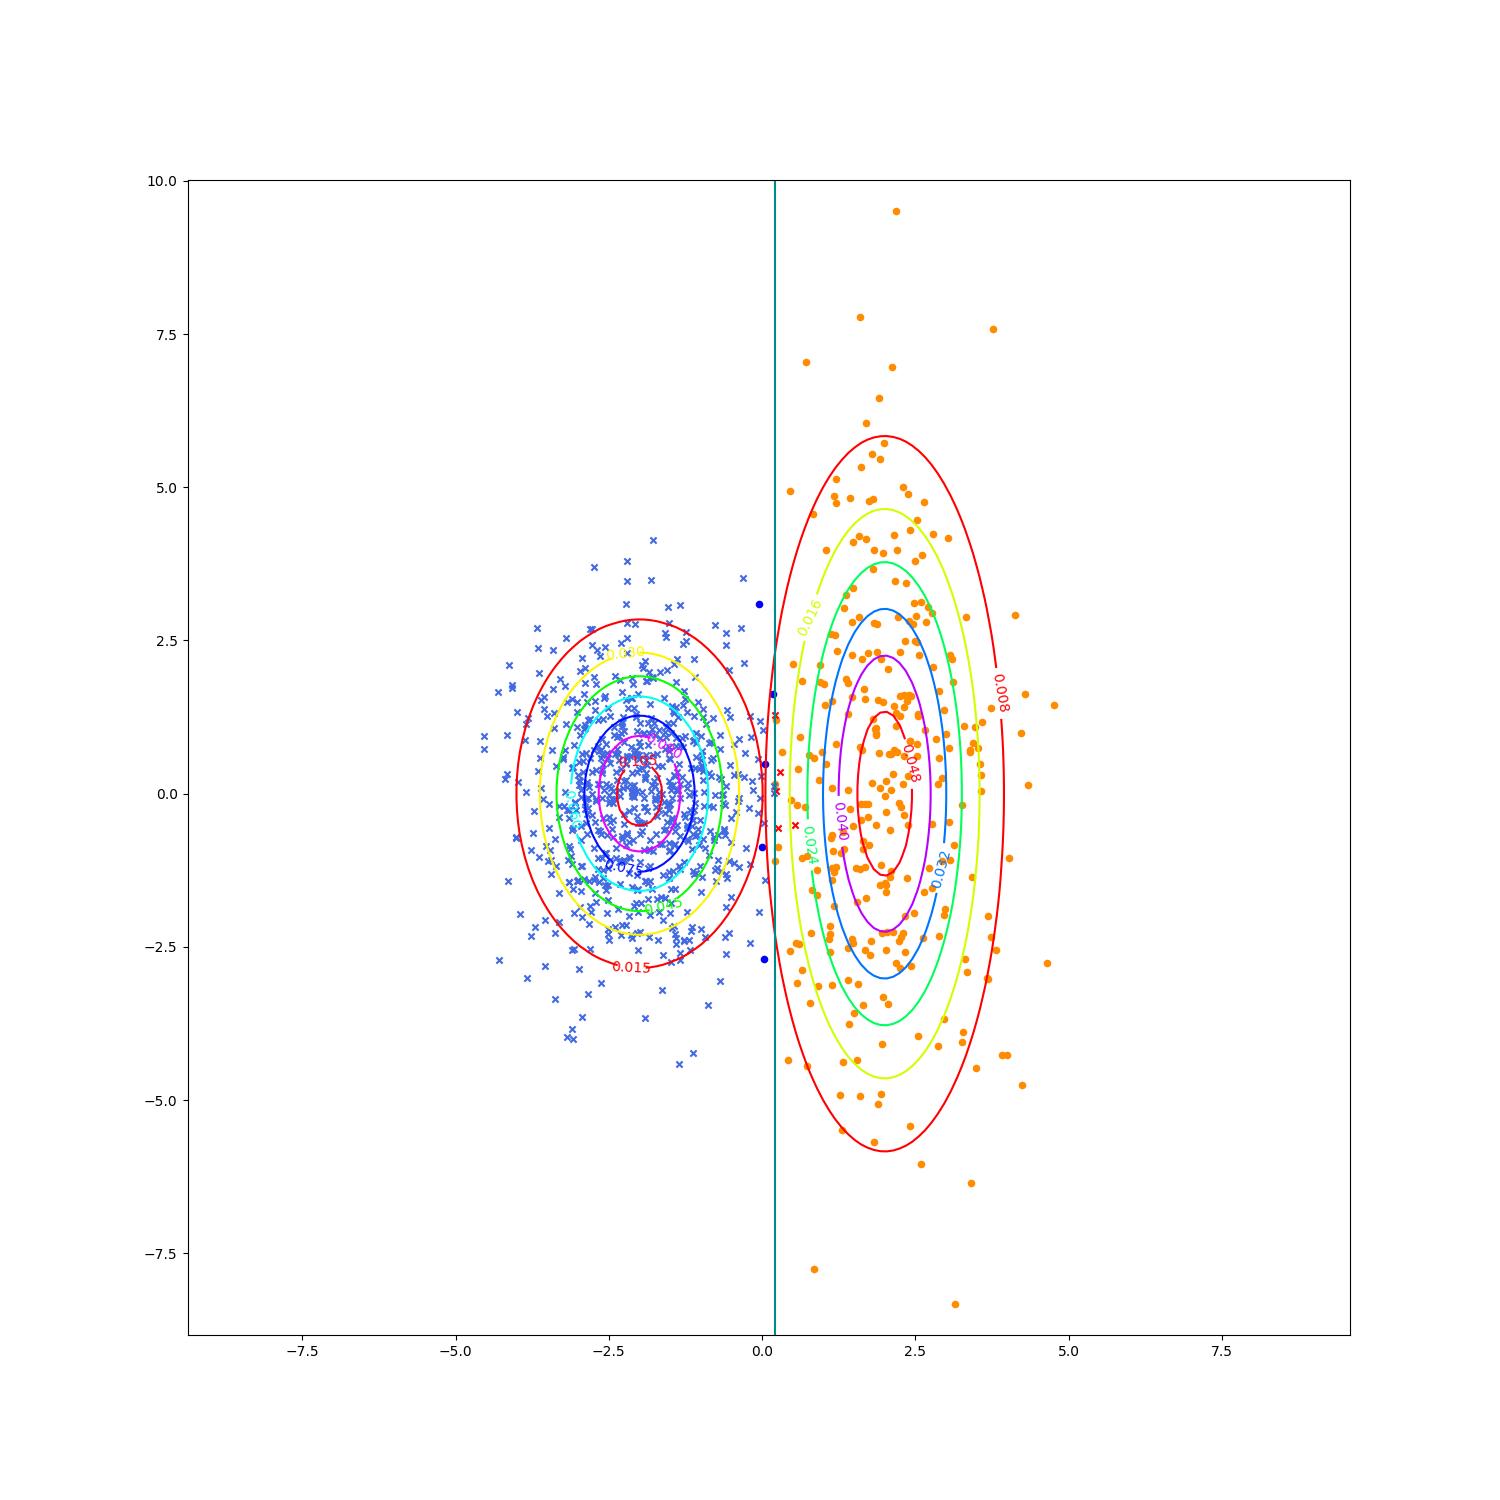
\includegraphics[clip, width=\linewidth]{../figures/result_assignment1_dataset1_case1.png}
    \caption{dataset 1に対してCase 1の識別関数を適用したときの散布図と識別境界線}
    \label{fig:result_dataset1_case1}
\end{figure}

\begin{figure}
    \centering
    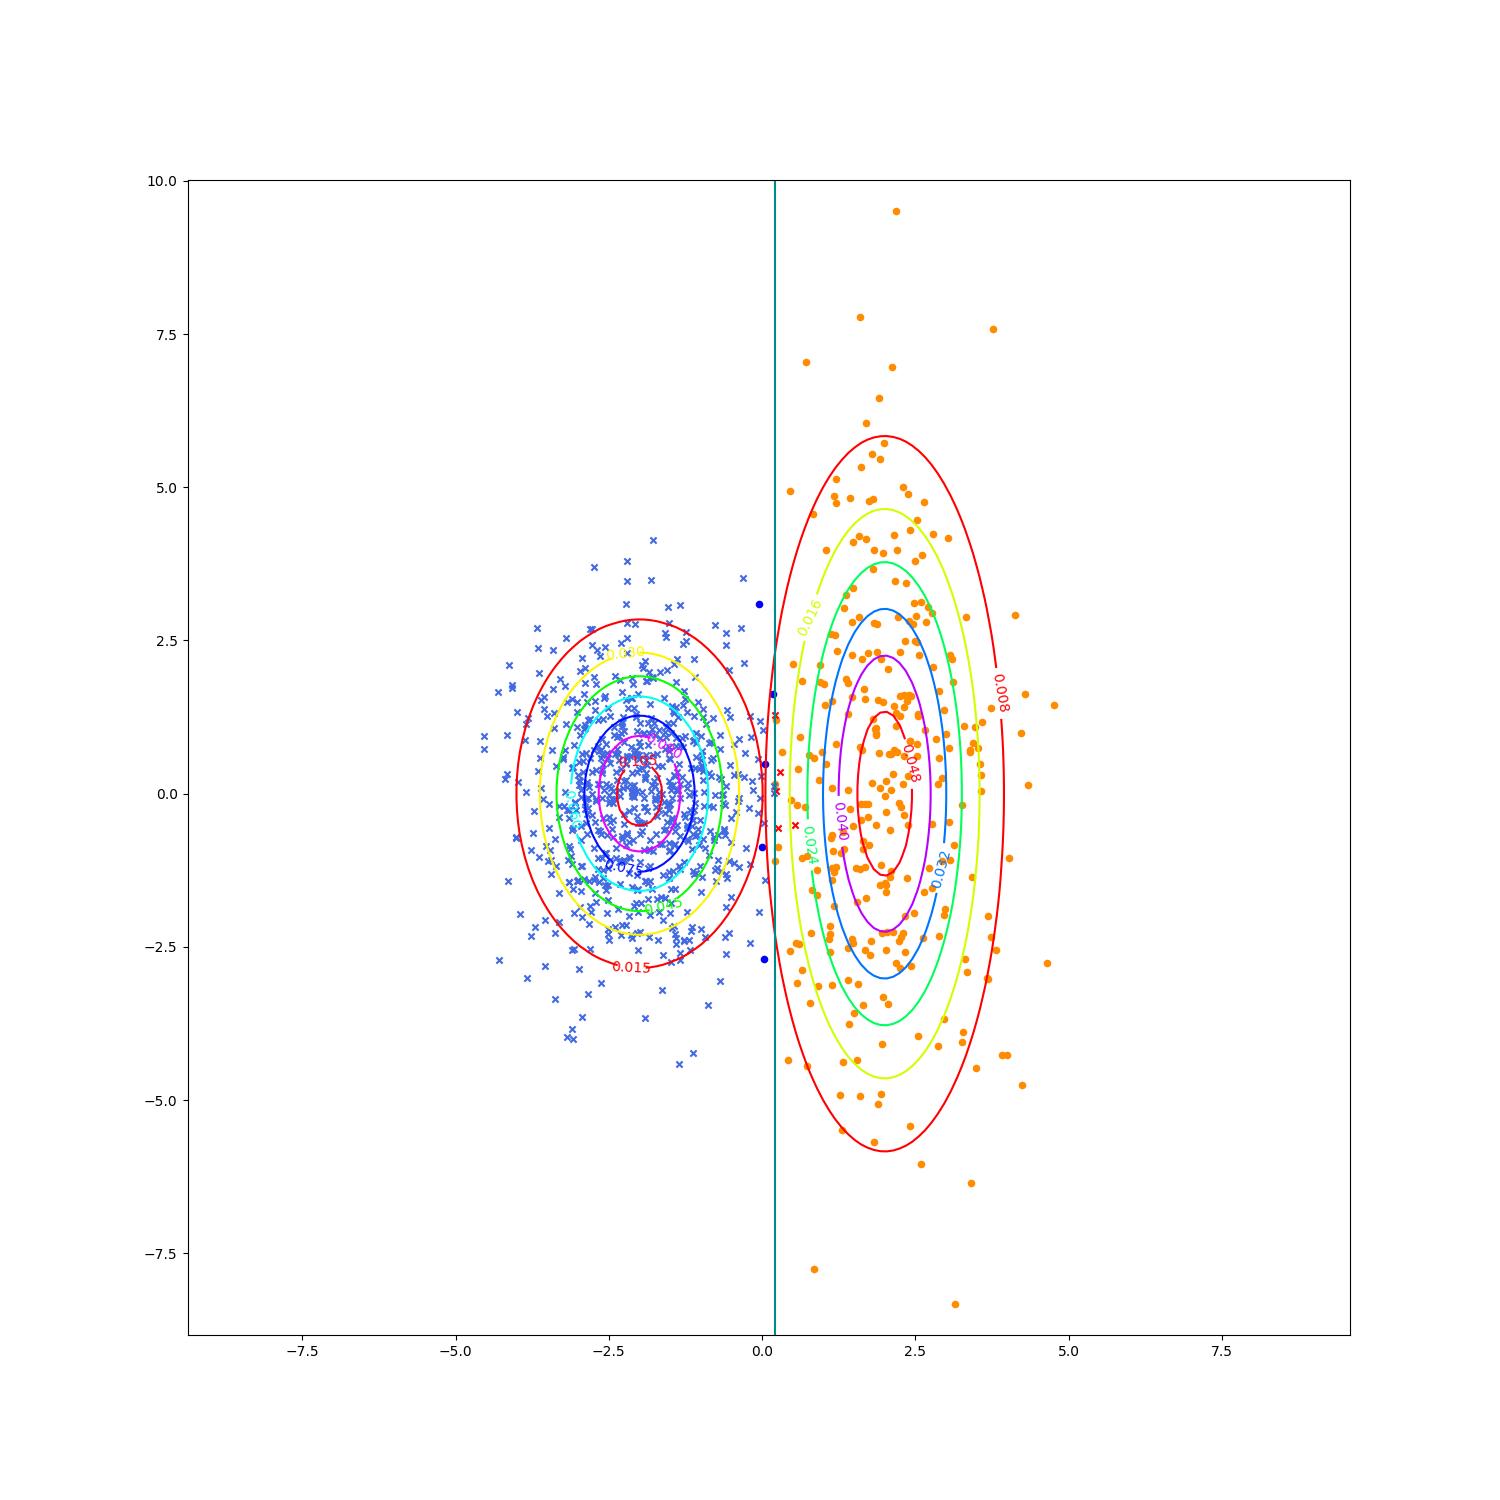
\includegraphics[clip, width=\linewidth]{../figures/result_assignment1_dataset1_case2.png}
    \caption{dataset 1に対してCase 2の識別関数を適用したときの散布図と識別境界線}
    \label{fig:result_dataset1_case2}
\end{figure}

\begin{figure}
    \centering
    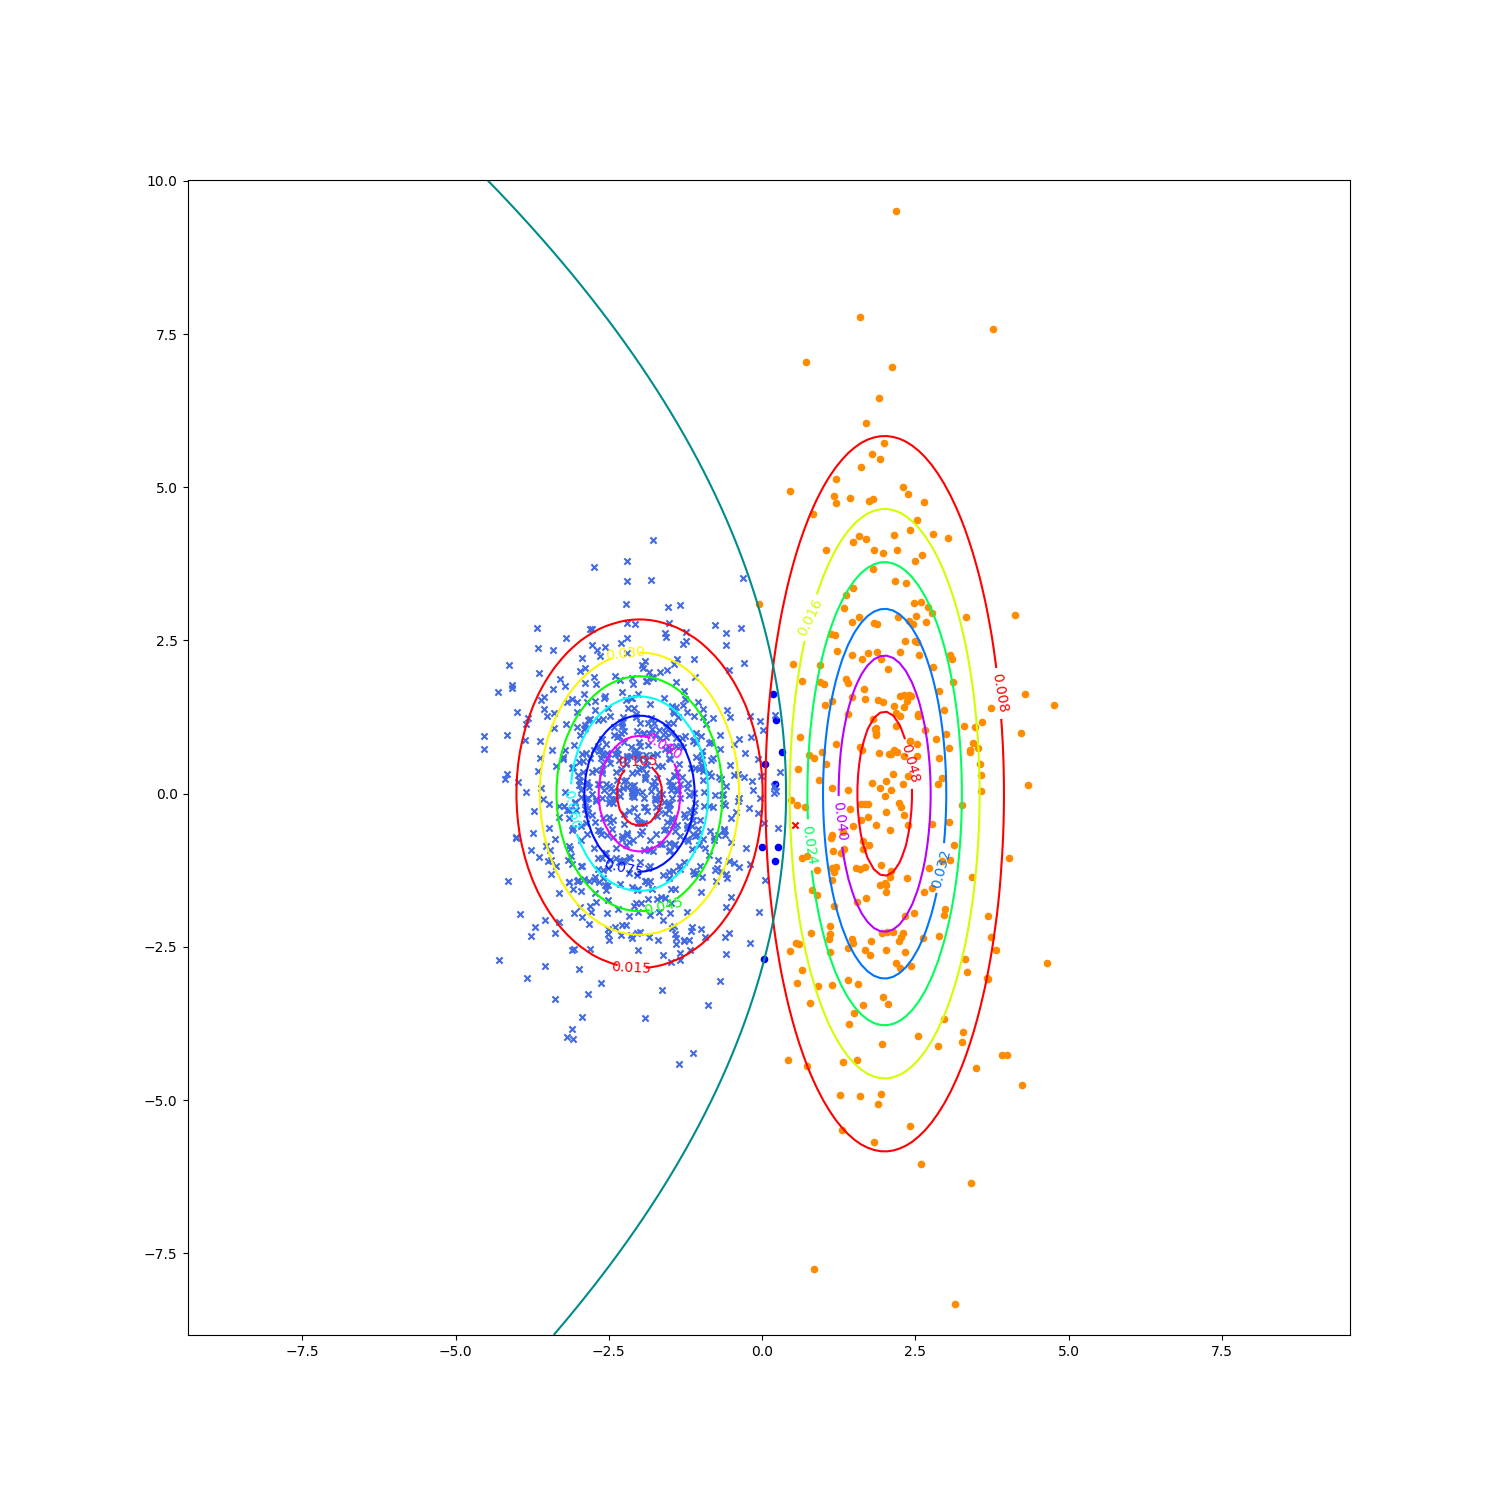
\includegraphics[clip, width=\linewidth]{../figures/result_assignment1_dataset1_case3.png}
    \caption{dataset 1に対してCase 3の識別関数を適用したときの散布図と識別境界線}
    \label{fig:result_dataset1_case3}
\end{figure}



\clearpage
\subsection*{dataset 2の結果}

\begin{table}[H]
    \centering
    \caption{dataset2に対する識別の結果}
    \begin{tabular}{lrrr}
            & Case 1 & Case 2 & Case 3 \\
        点群1の識別精度 & 370 & 357 & 361 \\
        点群1の識別精度 & 0.892 & 0.860 & 0.870 \\
        点群2の識別精度 & 540 & 549 & 550 \\
        点群2の識別精度 & 0.923 & 0.938 & 0.940 \\
        全体の正解率 & 0.910 & 0.906 & 0.911
    \end{tabular}
    \label{tab:dataset2_result}
\end{table}

\begin{figure}
    \centering
    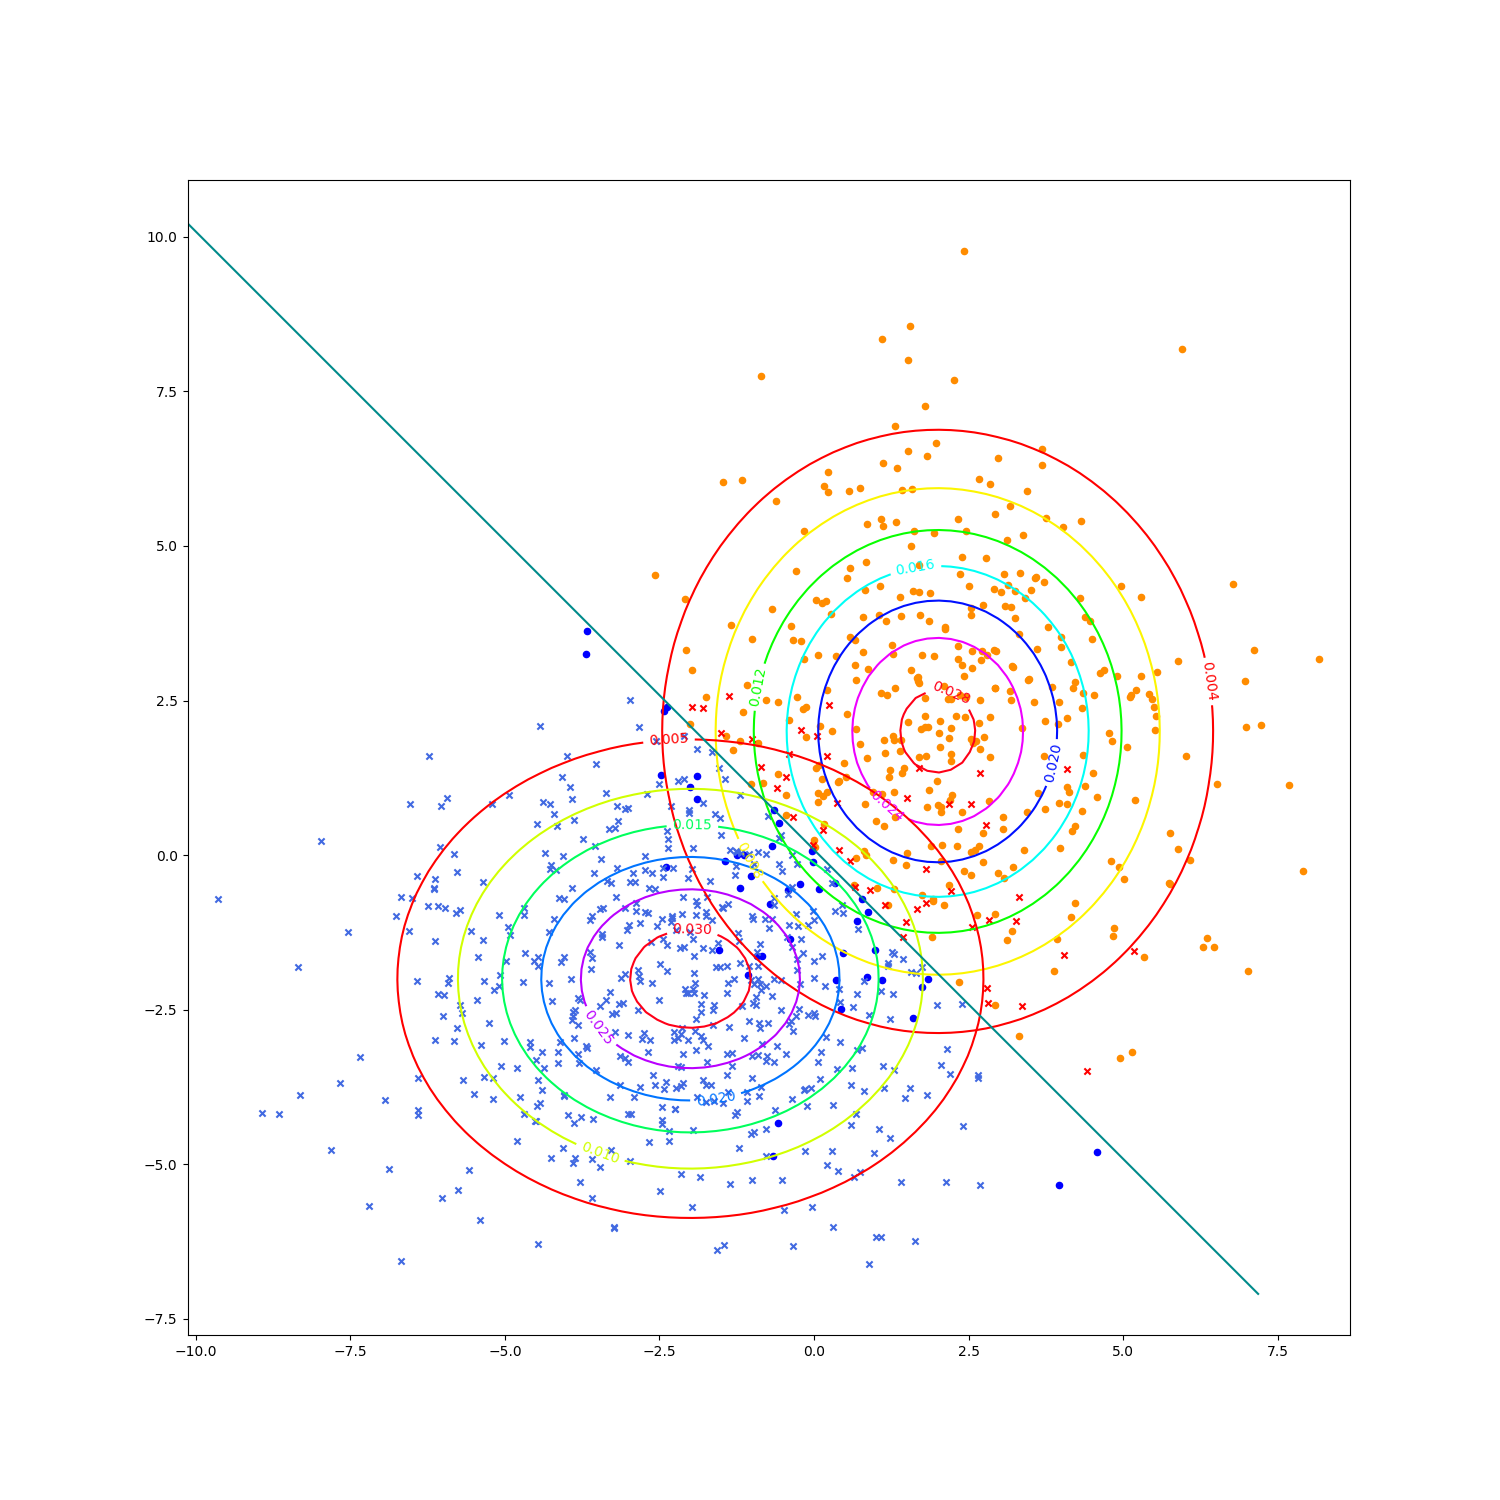
\includegraphics[clip, width=\linewidth]{../figures/result_assignment1_dataset2_case1.png}
    \caption{dataset 2に対してCase 1の識別関数を適用したときの散布図と識別境界線}
    \label{fig:result_dataset2_case1}
\end{figure}

\begin{figure}
    \centering
    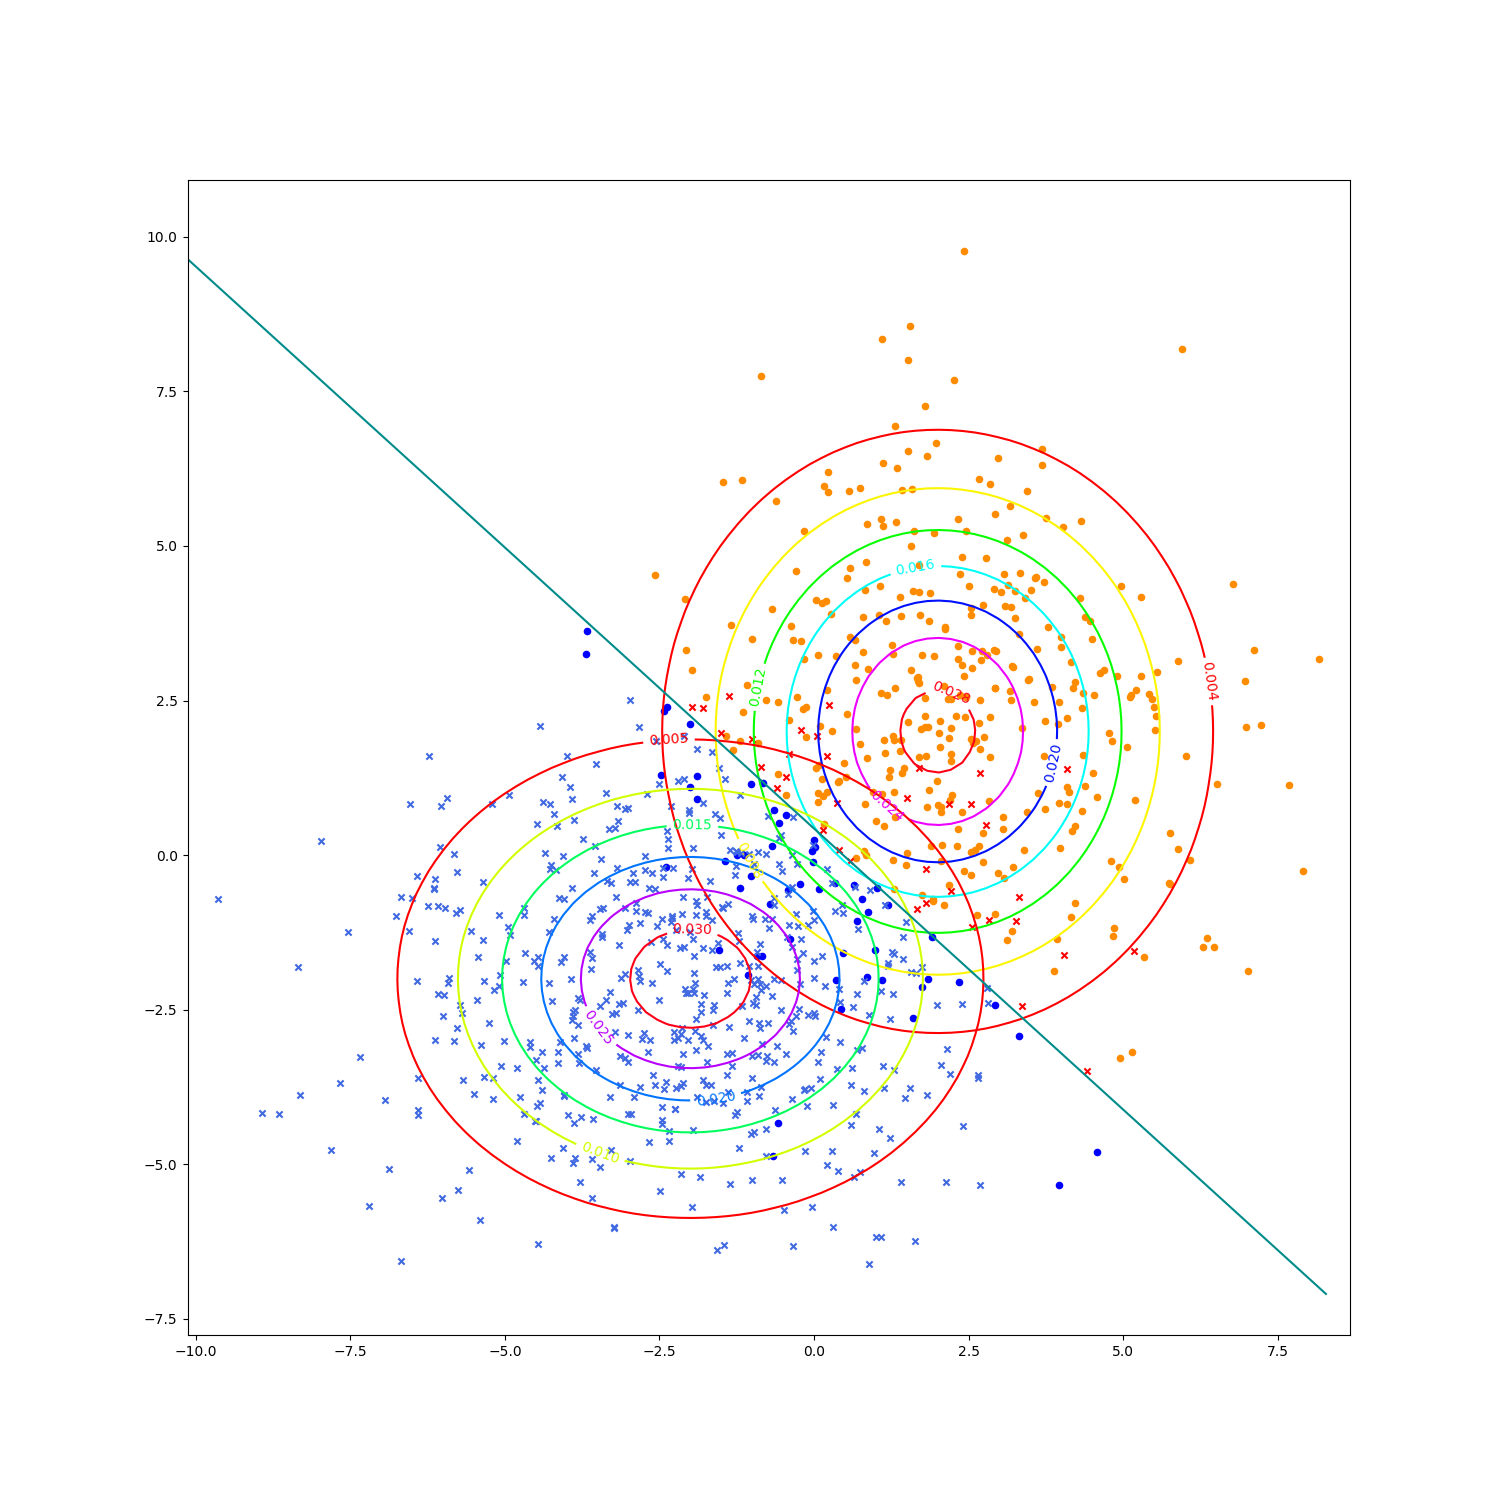
\includegraphics[clip, width=\linewidth]{../figures/result_assignment1_dataset2_case2.png}
    \caption{dataset 2に対してCase 2の識別関数を適用したときの散布図と識別境界線}
    \label{fig:result_dataset2_case2}
\end{figure}

\begin{figure}
    \centering
    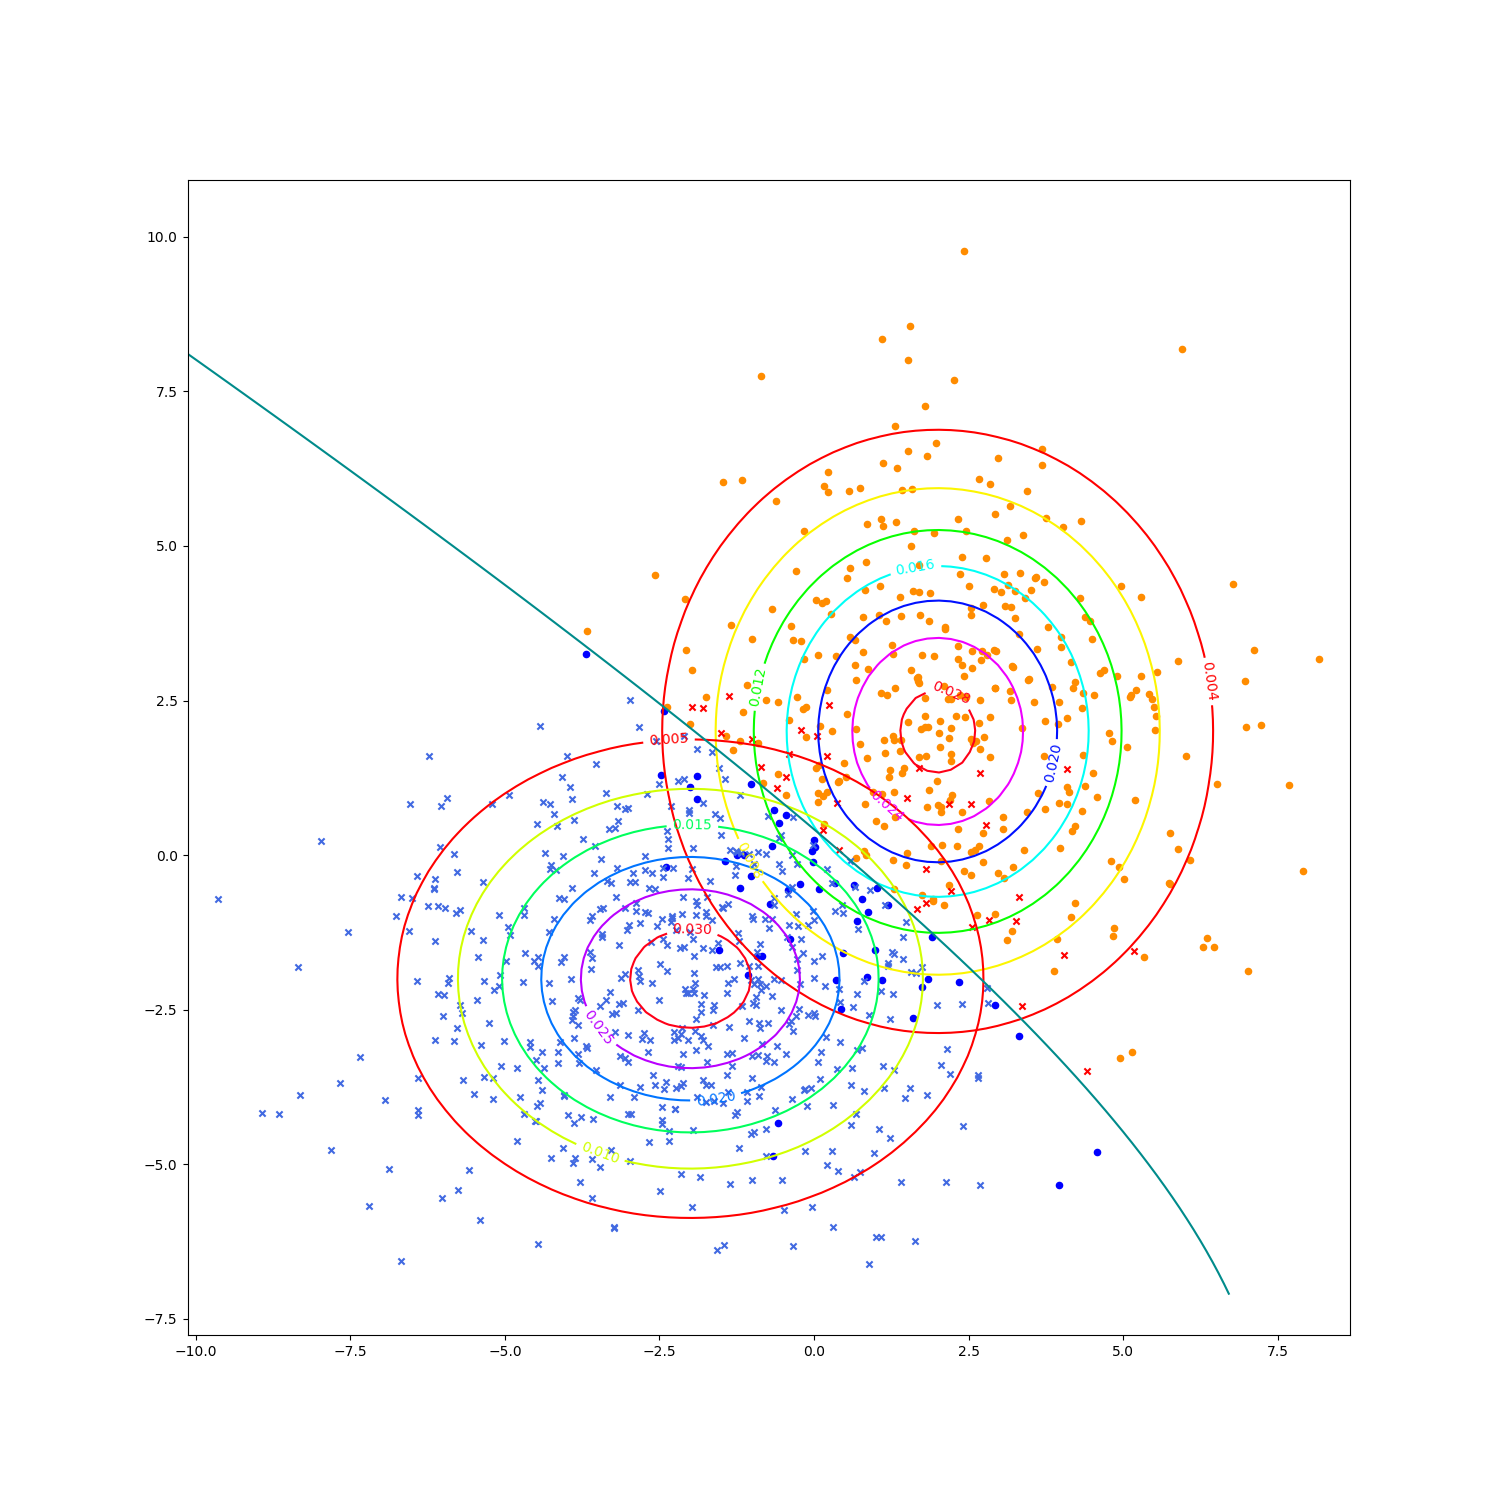
\includegraphics[clip, width=\linewidth]{../figures/result_assignment1_dataset2_case3.png}
    \caption{dataset 2に対してCase 3の識別関数を適用したときの散布図と識別境界線}
    \label{fig:result_dataset2_case3}
\end{figure}



\clearpage
\subsection*{dataset 3の結果}

\begin{table}[H]
    \centering
    \caption{dataset3に対する識別の結果}
    \begin{tabular}{lrrr}
            & Case 1 & Case 2 & Case 3 \\
        点群1の識別精度 & 517 & 517 & 465 \\
        点群1の識別精度 & 1.000 & 1.000 & 0.899 \\
        点群2の識別精度 & 0 & 0 & 295 \\
        点群2の識別精度 & 0.000 & 0.000 & 0.611 \\
        全体の正解率 & 0.517 & 0.517 & 0.760
    \end{tabular}
    \label{tab:dataset2_result}
\end{table}

\begin{figure}
    \centering
    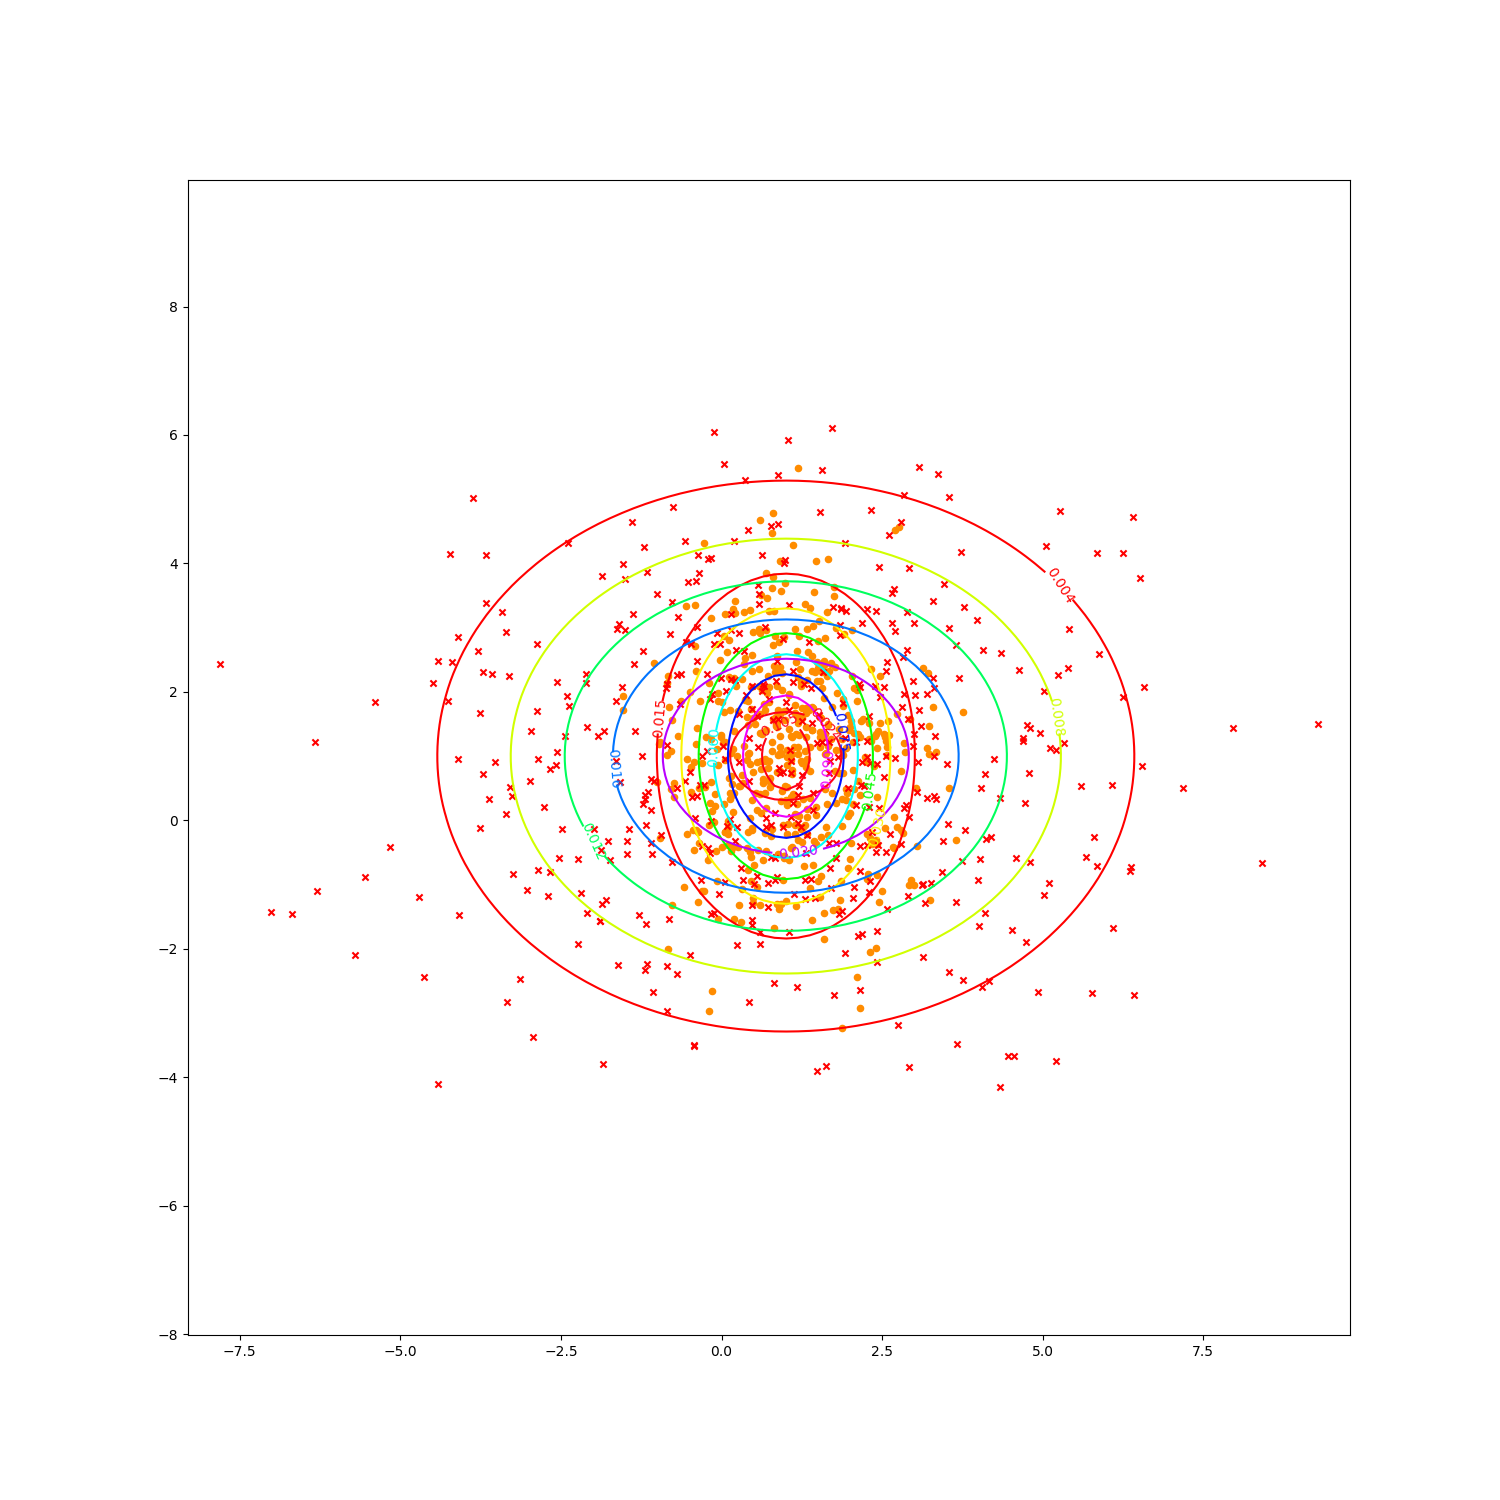
\includegraphics[clip, width=\linewidth]{../figures/result_assignment1_dataset3_case1.png}
    \caption{dataset 3に対してCase 1の識別関数を適用したときの散布図と識別境界線}
    \label{fig:result_dataset3_case1}
\end{figure}

\begin{figure}
    \centering
    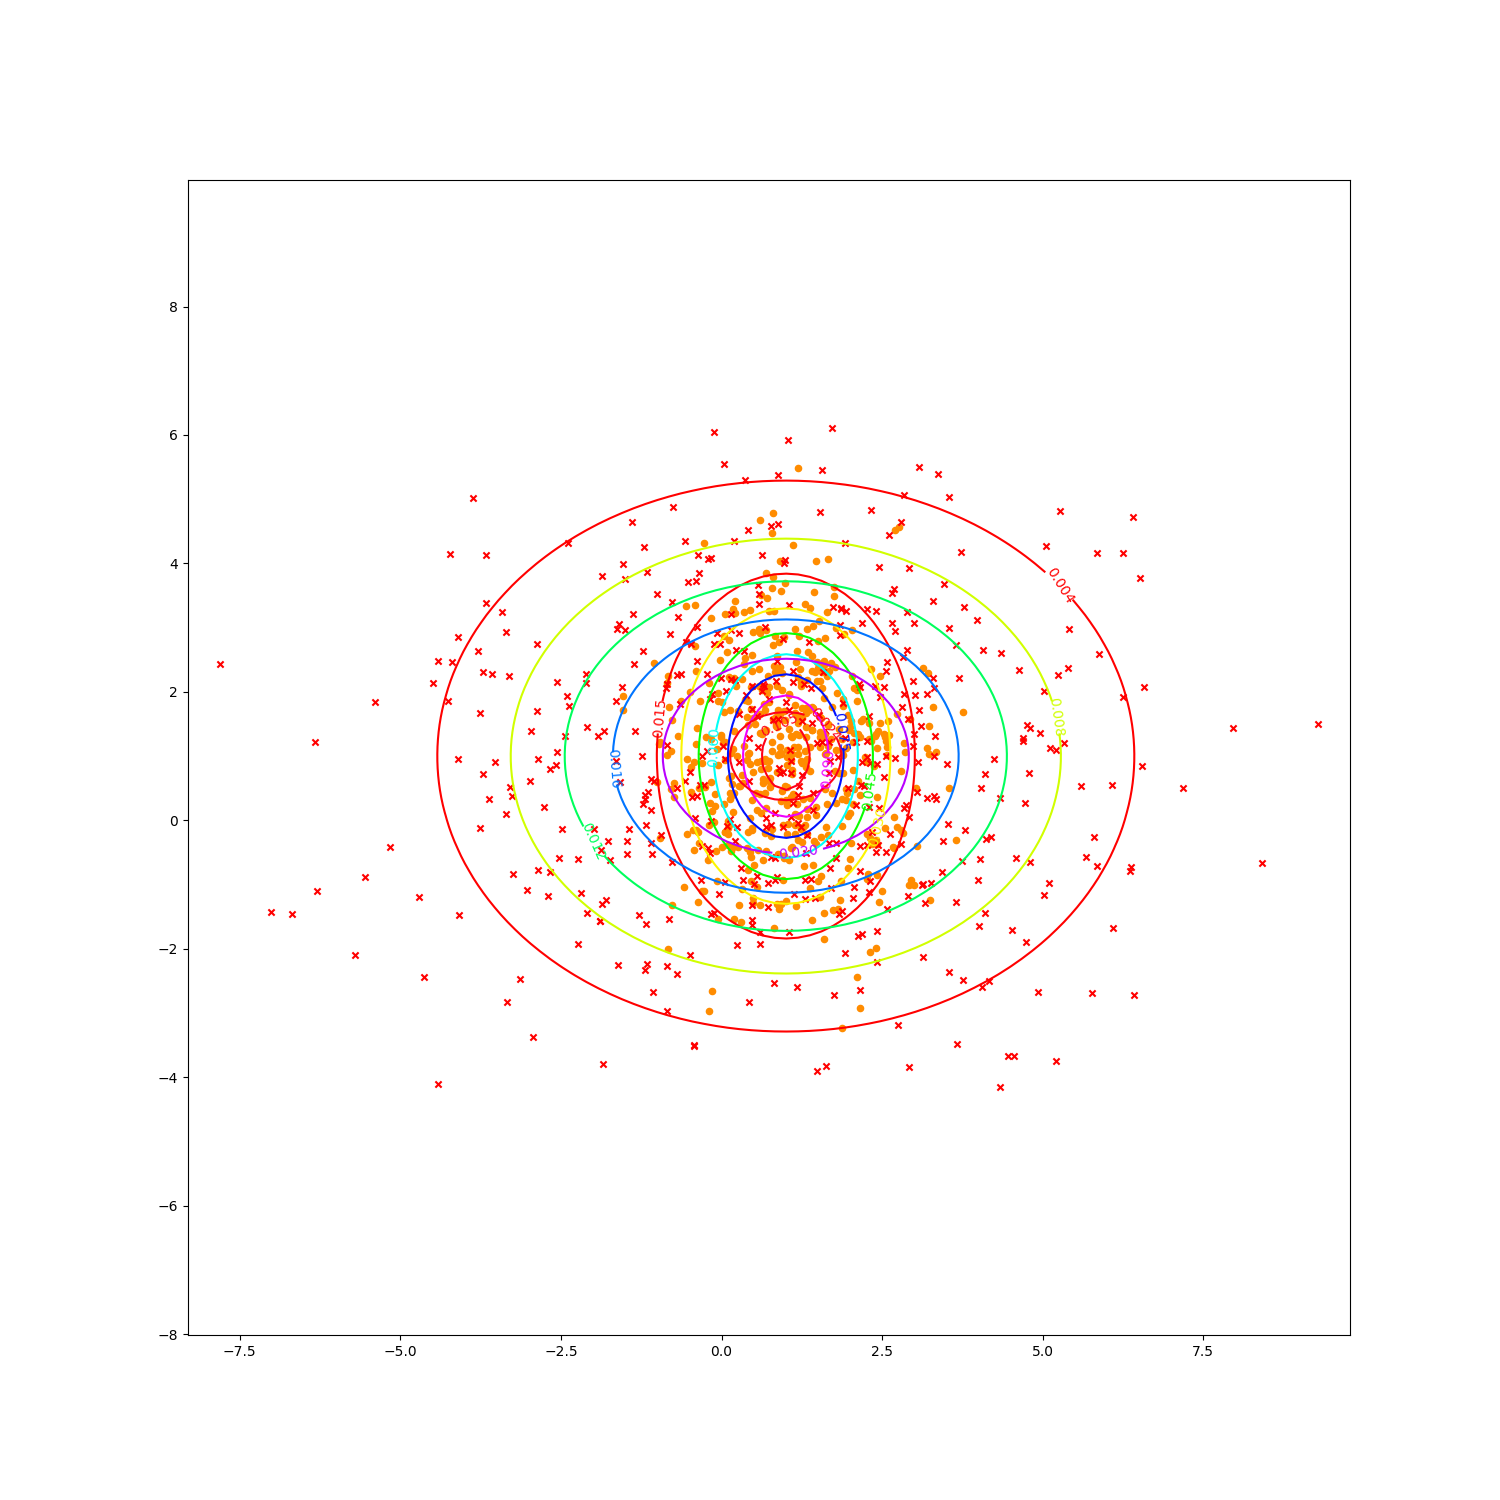
\includegraphics[clip, width=\linewidth]{../figures/result_assignment1_dataset3_case2.png}
    \caption{dataset 3に対してCase 2の識別関数を適用したときの散布図と識別境界線}
    \label{fig:result_dataset3_case2}
\end{figure}

\begin{figure}
    \centering
    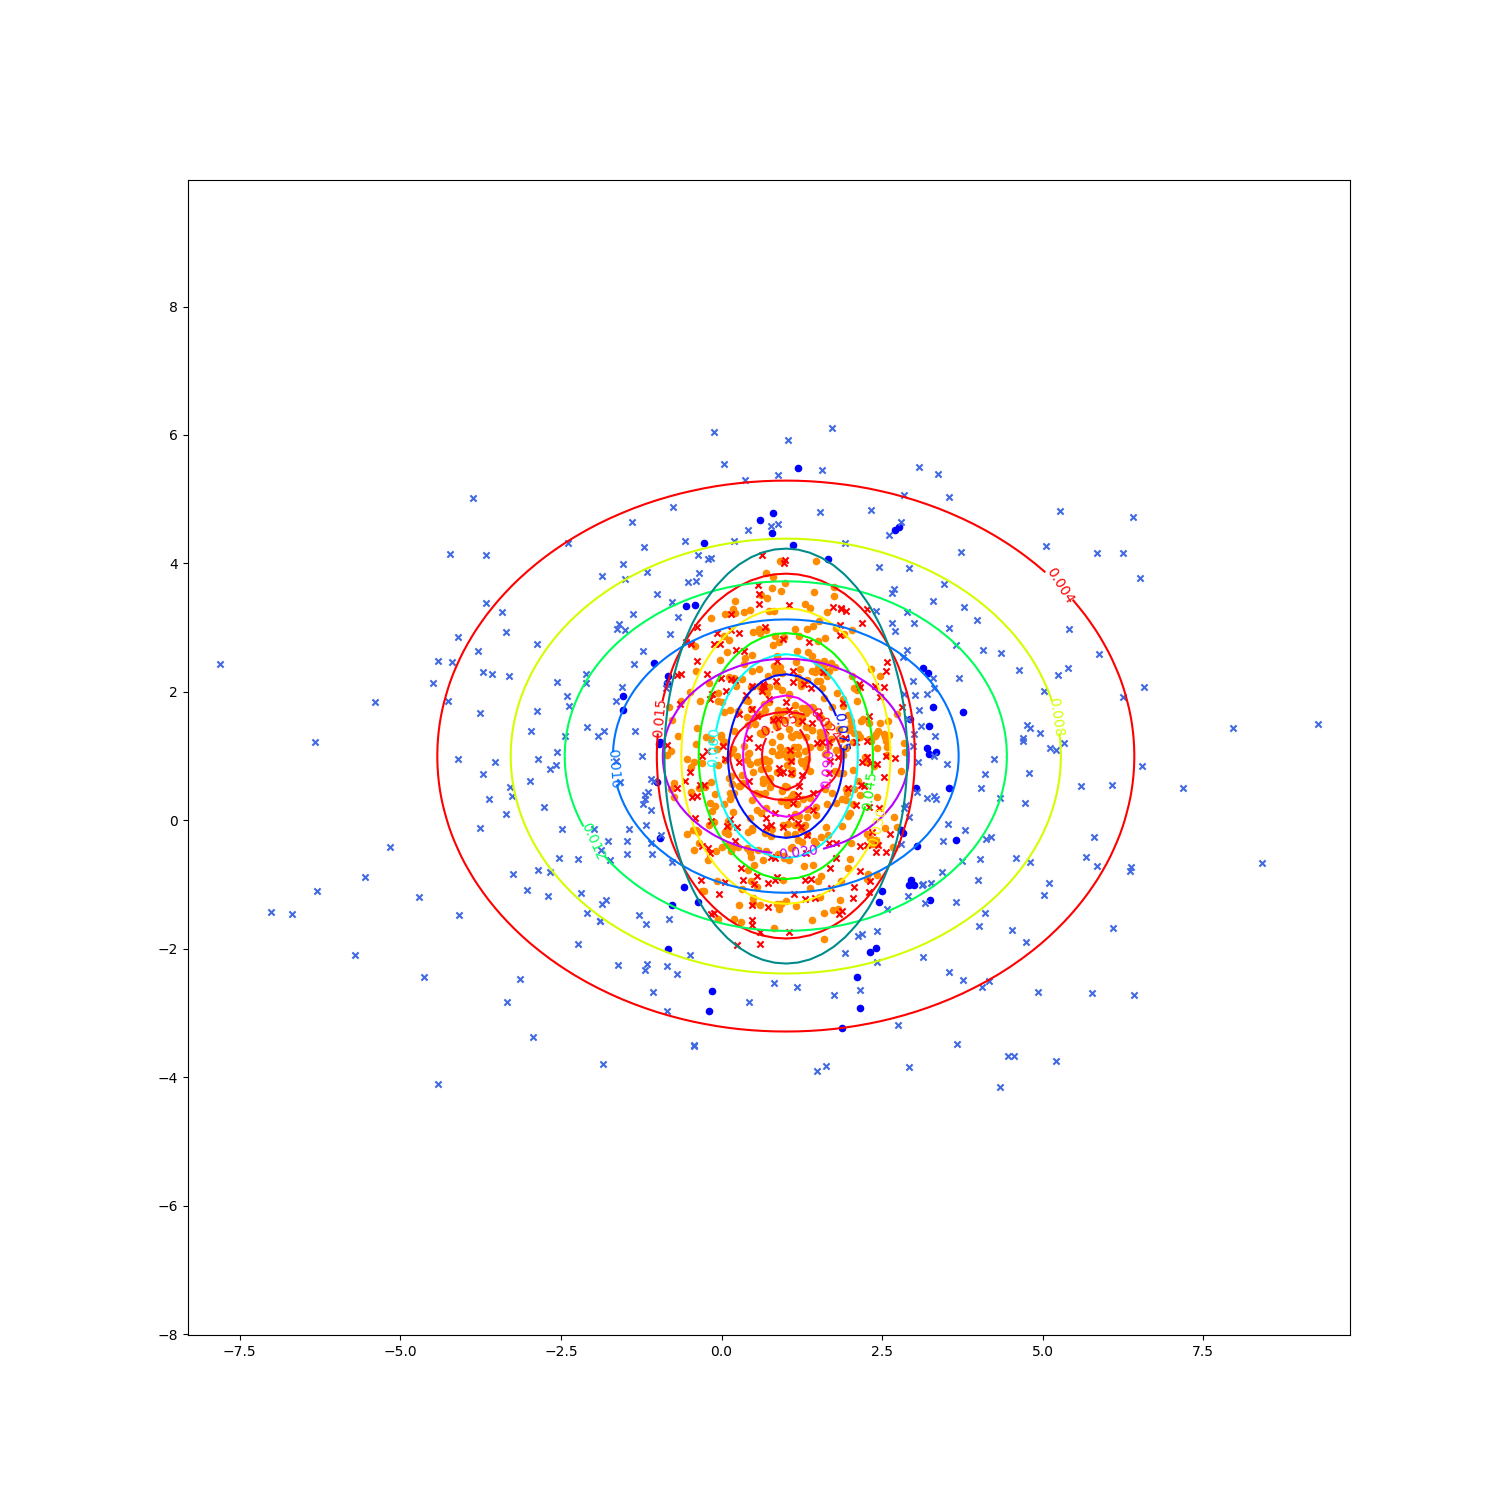
\includegraphics[clip, width=\linewidth]{../figures/result_assignment1_dataset3_case3.png}
    \caption{dataset 3に対してCase 3の識別関数を適用したときの散布図と識別境界線}
    \label{fig:result_dataset3_case3}
\end{figure}



\end{document}
